\documentclass[a4paper, 12pt]{article}
\usepackage[utf8]{inputenc}
\usepackage[margin=0.8in]{geometry}
\usepackage{graphicx}
\usepackage{textcomp}
\usepackage{setspace}
\usepackage{hanging}


\title{FIT3163 Project Design Specification}
\author{g}
\date{May 2020}

\begin{document}
\begin{titlepage}
\addtolength{\hoffset}{0cm}
	\centering
	
\includegraphics[width=0.90\textwidth]{monash1line.jpg}\par\vspace{2cm}
	{\LARGE\bfseries A data mining technique to detect coronary artery disease using predictive modelling \par}
	\medskip\medskip
	\hrule
	\vspace{3cm}
	{\Large\bfseries Yupeng (Vita) Miao \par
	\medskip
	Yunxuan Wang \par
	\medskip
	Chang Yu Wang \par}
    \vspace{3cm}
    
   {\Large\bfseries Monash University\\}
    \medskip
    \large\textbf{Faculty of Information Technology\\}
    
    \vspace{3cm}
     % Bottom of the page
	\large A Project Design Specification for \\
	\large  \textit {FIT3163 Group Project}\\
	\vfill
	{\large  May 2020}
\end{titlepage}
\doublespacing
\tableofcontents
%These sections are broken up corresponding to the rubric/
\pagebreak
\onehalfspacing
\section{Introduction}
Coronary artery disease (CAD) is caused by blockages in the arteries due to cholesterol and fatty build up and is one of the leading causes of death in developed countries. In Australia, it was the leading cause of death for all age groups, accounting for 11.5\% of deaths (18590) in 2017 alone. It is especially prevalent in the elderly population aged 45 and over (AIHW, 2019). Current methods of diagnosing coronary heart disease such as angiography are invasive and expensive, and so we are investigating the use of machine learning models to make a non-invasive diagnosis. This document outlines the high-level structure of our project, as well as outlining the processes and software we will use in each step.
%=====
\section{Architectural Design} %decompose into 2 layers or more
The bulk of the project is to create a predictive model for CAD and investigate the effectiveness of various statistical learning techniques such as, but not limited to, support vector machines, neural networks and random forests.
The best performing combination of models will be made into an API which users can ping, submitting a (partial) feature set and returning a result.
We will build a simple web application that uses the API and allows users to do this without coding knowledge, which will have simple diagrams and possible suggestions. See figure \ref{fig:overall_flowchart} for details.

\begin{figure}[h]
    \centering
    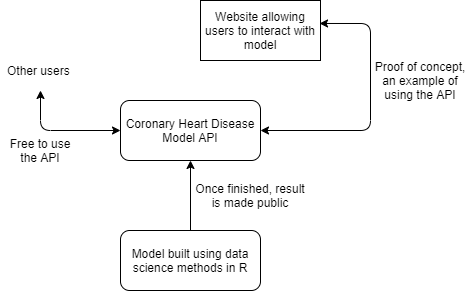
\includegraphics[width=0.8\textwidth]{Diagram1.png}
    \caption{A high level representation of the project. The core deliverables are the rounded bubbles, and the rectangle is a planned extra feature.}
    \label{fig:overall_flowchart}
\end{figure}We will then use R and various packages detailed below to take the input of the given data set and output a predictive model.

\subsection{Data Collection and Processing}
We will use standard data science methods throughout the entire process. A summary of the methods can be found in figure \ref{fig:model_summary}.
\subsubsection{Data set}
The primary data set will be the one collected by Alizadehsani et al. (2013), which comprises of 303 patients with 54 features for each subject. These features are used for heart disease prediction and detection. We may also use secondary data sets from other online sources, such as cadata set.com and the UCLA database.
\begin{itemize}
    \item \underline{cadata set.com} This provides a comprehensive data set about the machine learning research on CAD.
    \item \underline{UCLA database} The University of California Los Angeles library also provides a number of database related to CAD. 
\end{itemize}
After a preliminary research about the potential data set we may use, we found that the related data sets are either have a large number of observations with very limited features or contains plentiful features with a small sample size. Usage of data sets with very limited features may reduce the prediction accuracy due to the omitted variable bias, while using a small data set with plentiful features may introduce more variance in the model as the sample size is fairly small.\\\\
Furthermore, each individual dataset samples participants from a limited number of countries, with the majority of these being from a single country. This means that a classifier trained on a single dataset may only apply to a limited population. Our group will train different classifiers using various datasets so that we can make this tool be accessible to the greater population. 

\subsubsection{Data Wrangling}
The data wrangling involves the following steps:
\begin{enumerate}
    \item \underline{Restructuring:} Dummy variables will be derived from any multi-classed features, so that they can be used in fitting a logistic regression and other models.
    \item \underline{Remove/Changing Missing Values and Outliers:} Instead of simply removing the observations with null values, we will consider replacement with the feature's average/median values (numerical predictors) or more complex unsupervised learning algorithms (e.g. imputation) to deal with the missing values and outliers in the data set. 
    \item \underline{Enriching:} Following the approaches described in Alizadehsani et.al. (2013), our group may also derive extra useful features from the data set. 
\end{enumerate}

\subsection{Modelling Techniques}
Our plans on the classifier construction and model evaluation methods are described in this section. After data wrangling, our group will implement different combinations of feature selection approaches and classification algorithms to train the classifiers and measure those models' performance based on various criteria.
\subsubsection{Classification Algorithms}
We will explore the following classification algorithms in the project.
\begin{itemize}
    \item \underline{Logistic Regression:} Logistic regression has been used in biological science in the early $20^{th}$ century (Qi, 2013) and it is useful for modeling binary responses, such as if a patient has CAD. However, the features in the data may be correlated and so we will also explore methods that take this into account, such as Generalised Estimating Equations (GEE) or using Singular Value Decomposition. Moreover, our group will try Lasso regressions to help minimise the out of sample error. This can also incorporate feature selections as it can estimate coefficients to be zero.
    
    \item \underline{Naïve Bayes:} This is easy to implement but has the drawback of assuming that the predictors are independent, which is unlikely to be true for our data set. However, it has been used in other related studies and has achieved relatively high accuracy, our project will investigate it combining with decision trees.
    
    \item \underline{Support Vector Machines(SVM):} Our group members are not as familiar with this, but since it has been used to remarkable effect in related research (Alizadehsani et al., 2013), we will also train a SVM using Sequential Minimal Optimisation(SMO) algorithm after carrying out further studies on this method.
    
    \item \underline{Decision Trees:} The major advantage of decision tree over other regression methods is that it makes few assumptions about the data. We discuss the approach to growing the tree in the feature selection section below. However, it can be difficult to find a good tree and can be potentially unstable as it is likely to have high variance. This can be combated with random forests. Our group will also investigate the bootstrapping for sampling to mitigate its drawbacks.
    
    \item \underline{Neural Networks:} Neural Networks are a very powerful approach to modelling. Numerous studies referenced in Alizadehsani et al. (2013) used neural network classification algorithms in predicting CAD and showed promising accuracy.
    
\end{itemize}
    Ensemble learning algorithms have become very popular in recent times as it helps to improve the prediction results by running multiple models, overcome the common issue of over-fitting. In this project, we will also explore the effectiveness of various bagging and boosting algorithms.
    
\begin {itemize}
    \item \underline{Bagging: Random Forests} Modern biological science has shown an increasing use of random forests, which has a high prediction accuracy over large scale and complex data sets. Random forests helps to overcome the greedy nature of forward search in a single decision tree and can retain low bias and reduce the variance at the same time. Moreover, the random forest is more stable than growing a single decision tree. The feature selection is also incorporated in the learning process, but since this algorithms will fit multiple models, it may require more computation power depending on the number of splits.
    \item \underline{Boosting:} Different from Bagging that runs multiple models in parallel fashion, boosting trains multiple models in sequential fashion. Boosting has become quite popular in many data science competitions and has been used in many recent works in biological science. In this project, our team will train classifiers by implementing various boosting algorithms, including Adaptive boosting, Gradient boosting and XGBoost.
    \item \underline{Other Methods:}
    Our team will also train classifiers using unsupervised learning algorithms, such as K-nearest Neighbours(KNN) which has very few assumptions of the data.
\end{itemize}
\subsubsection{Feature Selection}
We will discuss forward selection, pruning approaches, (k-fold) cross validation, and weights in SVMs.
\begin{itemize}
  \item \underline{Forward selection} starts with an empty model and, in each  step, adds the variable which most improves the classifier according to information criteria.
  
  \item \underline{Pruning approach} starts with a full model and, at each step, removes the variable which least weakens the model in terms of the information criteria.
  
  The information criteria include Akaike Information Criterion (AIC), Bayesian Information Criterion (BIC) and Kullback information criterion (KIC), where AIC and KIC are recommended for analysis with a large number of possible predictors. Both the forward search and pruning approach are step-wise selection techniques which have a greedy nature. This can be overcome with algorithms that run multiple models with different initial conditions, such as random forests.

    \item \underline{Bonferroni Procedure:} For the logistic regression, the Bonferroni procedure, which is a very conservative approach, is also considered.
    \item \underline{Weights by SVM:} This procedure was considered in Alizadehsani et al. (2013), so our group will also investigate this approach in our project.

    \item \underline{(K-fold) Cross Validation:} This involves partitioning the data into $k$ partitions, fitting models to all but one of the partitions and testing the accuracy on the remaining. The resulted is used to improve the model and can be repeated k-times.
\end{itemize}

\begin{figure}[ht]
    \centering
    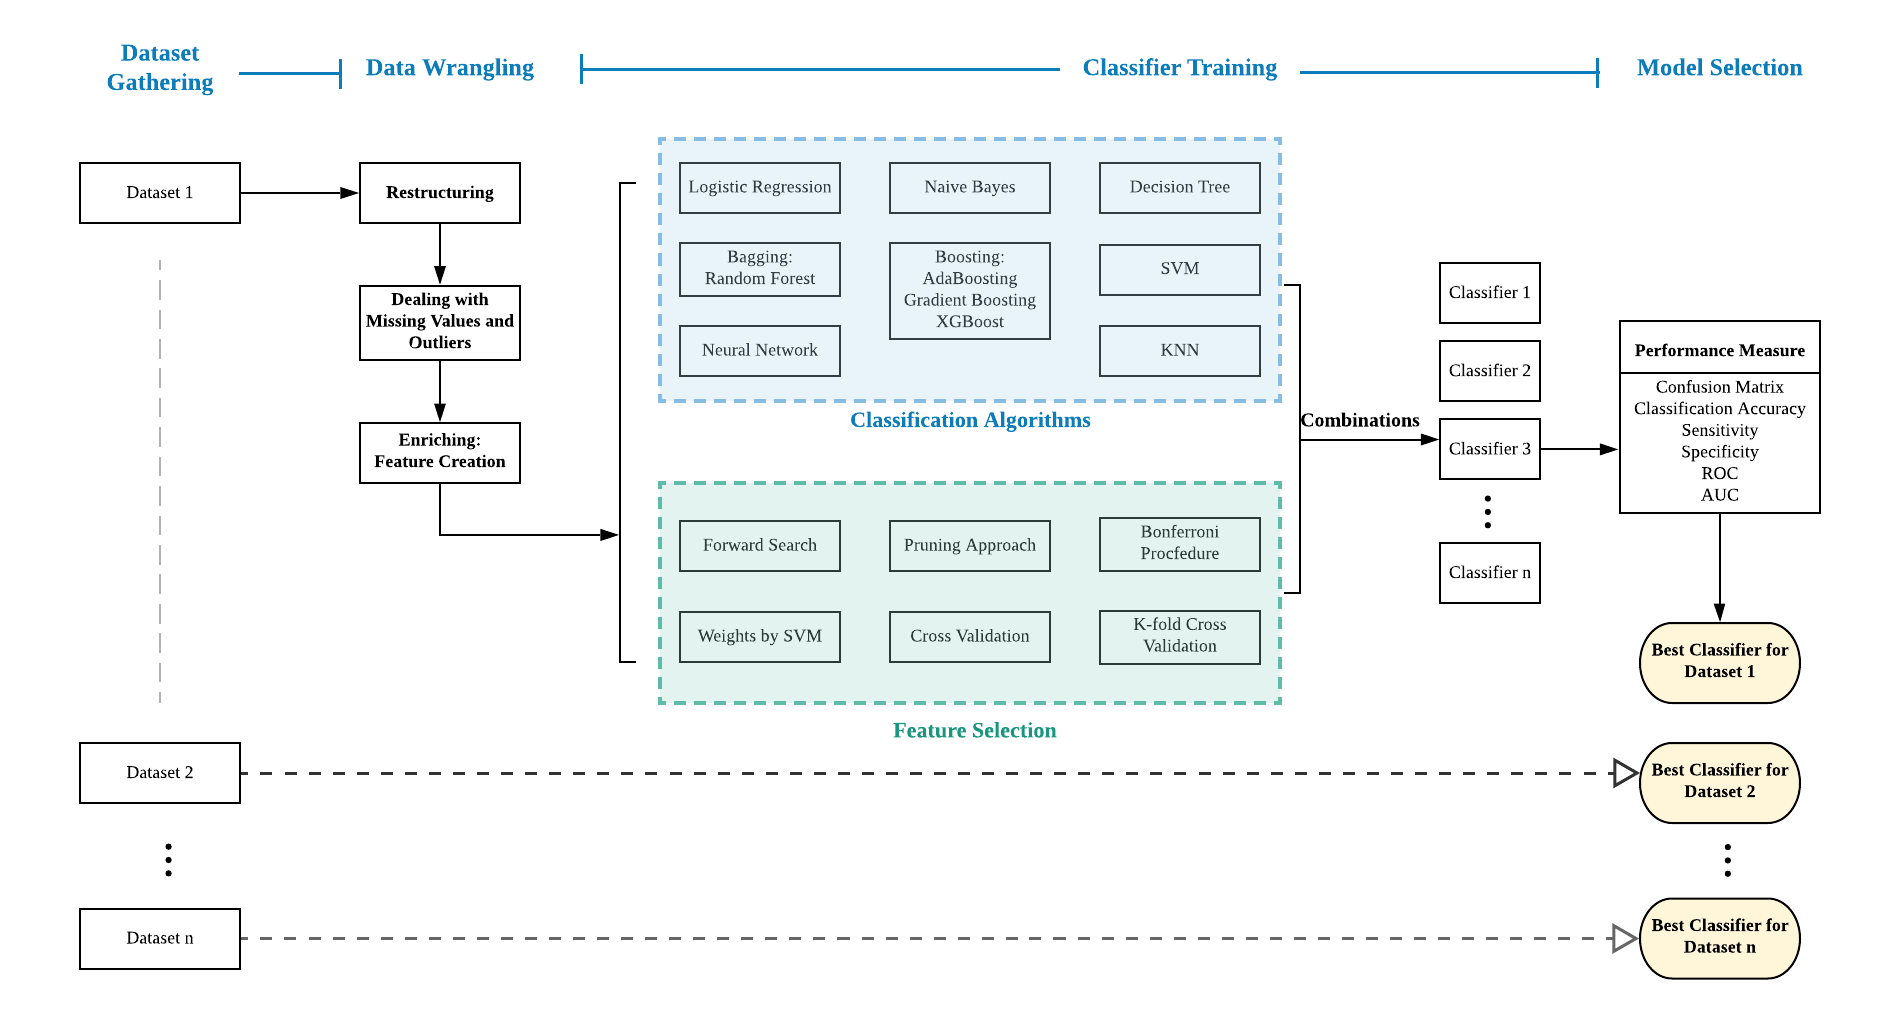
\includegraphics[width=1\textwidth]{Model.png}
    \caption{A summary of the model building process, from data gathering to model selection. Note that we will not do all combinations of classification algorithms and feature selection, instead taking the most effective methods for each algorithm.}
    \label{fig:model_summary}
\end{figure}

\subsubsection{Performance Measures}
Classification accuracy, sensitivity and specificity are considered to be the most important criteria for performance (Alizadehsani et al., 2013). Therefore, we will evaluate the performance of the classifiers based on the confusion matrix, classification accuracy, sensitivity and specificity and area-under-the-curve (AUC). Moreover, we will also consider the Receiver Operating Characteristics (ROC).

\subsection{The API}
We will host the API either on a personal device, or a cloud service such as Amazon Web Services or GitHub. Users can request a prediction from this API by sending a data point containing values for each feature, such as age and weight. The API will return a prediction, as well as additional information such as how this data point compares to the training set.

\subsection{The Website}
The website will be a simple UI that allows users to input data, allowing users to make a request to the API without any technical knowledge. 

\subsection{Justifications}
As data science students, our focus is to create a strong model for CAD. We will compare and contrast many different modelling techniques to gain a baseline understanding before combining them to create a more accurate model. An API is the best way to showcase the result, and allows users to test the model and interface with it seamlessly. Finally, the website is essentially a proof of concept, giving an example of how the API can be used. As we are unfamiliar with the technical side of APIs and front-end development, we will need to up skill to complete these. We may run into stability or performance issues with the API and website.

%===== 
\section{Software Specifications}
\subsection{Software Used}
\begin{itemize}
    \item \underline{Website development:}We will adopt the MERN framework, replacing components as necessary. MERN is an effective JavaScript framework that allows a seamless transition between components of full stack development. This serves as a good starting point as we are relatively inexperienced in this area.
    
    \item \underline{Model construction:}All the classifier training will be conducted using the R language on R Studio.
\end{itemize}
\subsubsection{R libraries}
We will use the many R libraries to develop models, such as tidyverse, dplyr, ggplot2, caret, mlr and shiny. The packages that are used for implementing those machine learning algorithms mentioned above are specified as following:
\begin{itemize}
    \item \underline{Naïve Bayes:} h2o, naivebayes
    \item \underline{Logistic Regression:} glmnet
    \item \underline{Support Vector Machines:} e1071, pathClass, penalizedSVM
    \item \underline{Decision Tree:} tree, rpart
    \item \underline{Neural Network:} nnet, neuralnet, brnn
    \item \underline{Random Forest:} randomForest
    \item \underline{Boosting:} mboost, xgboost
    \item \underline{K-nearest Neighbours:} knn(function)
    \item \underline{Stepwise regression:} leaps
\end{itemize}
\subsubsection{API software}
The R package `plumber' will likely be used to host the API, as it can be done directly in R studio (Allen, 2018).

\subsubsection{Website}
We will likely create a simple website with java script, hosted on a GitHub account. This is subject to change as our skill set changes throughout the project.

\subsection{Process Management Tools}
We will use a variety of tools to streamline and record our progress.
\begin{itemize}
    \item Zoom - for meetings.
    \item Messenger - to keep updated between meetings.
    \item Email - to send files keep a paper trail. 
    \item Overleaf - to produce any reports.
    \item GitHub - to collaborate on the code and maintain a change log.
\end{itemize}

\section{Concluding Remarks}
Our project aims to provide a less intrusive method to diagnose those at high risk of CAD. We  note that any results obtained from the model are not a substitute for professional medical advice. The tool is designed to be used in conjunction with expert knowledge from a medical professional.

\section{References}
\begin{hangparas}{0.7cm}{1}
AIHW (2019). Deaths in Australia, Leading causes of death - Australian Institute of Health and Welfare. Retrieved from https://www.aihw.gov.au/reports/life-expectancy-death/deaths-in-australia/contents/leading-causes-of-death

Alizadehsani, R., Habibi, J., Hosseini, M.J., Mashayekhi, H., Boghrati, R., Ghandeharioun, A., Bahadorian, B. and Sani, Z.A. (2013). A data mining approach for diagnosis of coronary artery disease. \textit{Computer methods and programs in biomedicine, 111}(1), 52-61. doi:10.1016

Allen, J. (2018). Creating APIs in R with Plumber. Retrieved from https://www.rplumber.io/
docs/index.html#web-apis

Qi, Y. (2012). \textit{Ensemble machine learning} (pp. 307-323). Boston, MA: Springer.
\end{hangparas}
\end{document}